\documentclass[a4paper,12pt,russian]{extarticle}
\usepackage{../MyPackages/commands}
\RequirePackage{caption}
\usepackage{graphicx}
\newcommand{\Pn}[3]{P^{(#1)} \br{#2,#3}}
\newcommand{\G}{\Gamma}
\newcommand{\e}{\eta_i^{(1)}}
\newcommand{\ee}{\eta_i^{(2)}}
\renewcommand{\b}{b^{(1)}}
\newcommand{\bb}{b^{(2)}}
\renewcommand{\P}[2]{P( #1 | #2)}
\newcommand{\iakt}{[\tau_{i},\tau_{i+1})}
\newcommand{\Gr}[1]{\Gamma^{(#1)}}
\newcommand{\Mark}{\{(\G_i, \vk_{1,i}, \vk_{2,i}, \vk_{3,i}, \vk_{4,i}); i \geqslant 0\}}
%\newcommand{\Markk}[0]{\brrr{ \vk_i, i \geqslant 0}}
%\newcommand{\Markkhat}[0]{\brrr{ \hat{\vk}_i, i \geqslant 1}}
%\newcommand{\Markkhata}[0]{\brrr{ \hat{\vk}_i\br{a}, i \geqslant 1}}
%\newcommand{\Markkhato}[0]{\brrr{ \hat{\vk}_i\br{0}, i \geqslant 1}}
%\newcommand{\Markkhatoa}[0]{\brrr{ \hat{\hat{\vk}}_i\br{a}, i \geqslant 1}}
\usepackage[Magistr]{../MyPackages/ptvstyle}
%\selectlanguage{russian}
\title{Моделирование и анализ системы обслуживания конфликтных потоков в классе приоритетных алгоритмов}
\author{студент группы 85М1\\ Кочеганов В.~М.}
\advisor{к.ф.-м.н., доцент \\ Зорин А.~В.}
\chief{д.ф.-м.н., профессор \\ Федоткин М.~А.}
\date{2014}
\newcommand{\p}{\hat{p}}
\newcommand{\gam}[2]{\Gamma^{\left( #1 , #2 \right)} }
\newcommand{\T}[2]{T^{\left( #1 , #2 \right)} }
\newcommand{\ga}[1]{\Gamma^{\left( #1 \right)} }
\newcommand{\Tt}[1]{T^{\left( #1 \right)} }
%\newcommand*{\hm}[1]{#1\nobreak\discretionary{}%
%{\hbox{$\mathsurround=0pt #1$}}{}}
\renewcommand{\Pr}{{\mathbf P}}
\usepackage{multicol}

\begin{document}

\section{Постановка задачи и построение математической модели}

\subsection{Постановка задачи на содержательном уровне}

Рассмотрим систему массового обслуживания следующего вида (Рис.~\ref{SystemScheme}).
\begin{figure}[h]
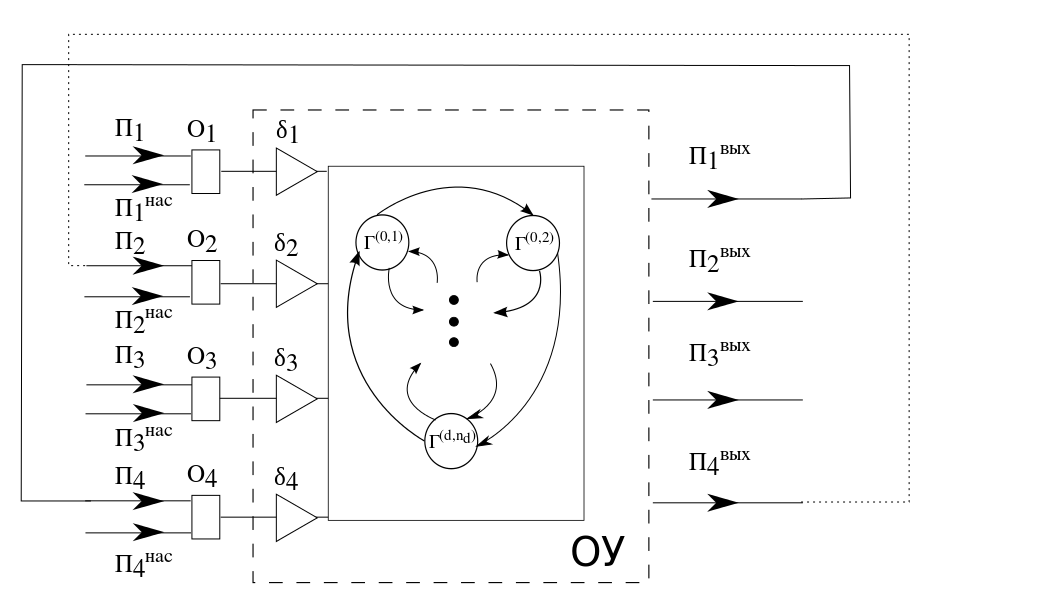
\includegraphics[scale=0.5]{SystemScheme.png} 
\caption{Структурная схема системы обслуживания}
\label{SystemScheme}
\end{figure}

Пусть в систему с одним обслуживающим устройством поступают потоки $\Pi_1$, $\Pi_2$, $\Pi_3$  и $\Pi_4$. Требования по потоку $\Pi_j$ становятся в соответствующую очередь $O_j$ с неограниченной вместимостью, $j\in \{1, 2, 3, 4\}$. Для $j \in \{1, 2, 3\}$ дисциплина очереди $O_j$, поддерживаемая устройством $\delta_j$, имеет тип FIFO (First In First Out). Таким образом, для обслуживания из соответствующей очереди выбирается то требование, которое пришло раньше. Дисциплина очереди $O_4$ будет описана ниже. Входные потоки $\Pi_1$ и $\Pi_3$ формируются внешней средой, которая, будем предполагать, имеет только одно состояние, то есть вероятностная структура потоков не меняется с течением времени. Требования потоков $\Pi_1$ и $\Pi_3$ формируют независимые между собой неординарные пуассоновские потоки, то есть  стационарные, без последействия и ординарные потоки групп требований. Интенсивности соответствующих простейших потоков для $\Pi_1$ и $\Pi_3$ будем обозначать $\la_1$ и $\la_3$, а распределение числа заявок в группе по потоку $\Pi_j$ будем описывать производящей функцией
\begin{equation}
f_j(z) = \sum_{\nu=1}^{\infty} p_{\nu}^{(j)} z ^{\nu}
\label{GeneratingFunc}
\end{equation}
которая предполагается аналитической при любом $z$ таком, что $|z|<(1+\varepsilon), \varepsilon > 0$. Величина $p_{\nu}^{(j)}$ определяет вероятность того, что по потоку $\Pi_j$ число требований в группе равно $\nu$, $j\in \{1,3\}$. Обслуженные требования потока $\Pi_1$ поступают на повторное обслуживание, формируя при этом поток $\Pi_4$. Потоки $\Pi_2$ и $\Pi_3$ являются конфликтными, что означает запрет на одновременное обслуживание требований этих потоков и, следовательно, исследование системы не может быть сведено к задаче с меньшим числом потоков. 
 
 В каждый момент времени обслуживающее устройство находится в одном из конечного множества состояний $\Gamma=\{\G^{(k,r)} \colon k=0,1,\ldots,d; r=1,2,\ldots n_k\}$ с заданными натуральными числами $d$, $n_0$, $n_1$, $\ldots$, $n_d$. В каждом состоянии $\ga{k,r}$ обслуживающее устройство находится в течение времени $\Tt{k,r}$. Введем множества $\G^{\mathrm{I}}$, $\G^{\mathrm{II}}$, $\G^{\mathrm{III}}$ и $\G^{\mathrm{IV}}$ следующим образом. В состоянии $\gamma \in \G^{\mathrm{\Rmnum{1}}}$ обслуживаются только требования из очередей $O_1$, $O_2$ и $O_4$.
В состоянии $\gamma \in \G^{\mathrm{\Rmnum{2}}}$ обслуживаются только требования из очередей $O_2$ и $O_4$.
В состоянии $\gamma \in \G^{\mathrm{\Rmnum{3}}}$ обслуживаются только требования из очередей $O_1$, $O_3$ и $O_4$.
В состоянии $\gamma \in \G^{\mathrm{\Rmnum{4}}}$ обслуживаются только требования из очередей $O_3$ и $O_4$.
Тогда множество $\G$ есть объединение $\G = \G^{\mathrm{I}} \cup \G^{\mathrm{II}} \cup \G^{\mathrm{III}} \cup \G^{\mathrm{III}}$ непересекающихся подмножеств. 

Смена состояний обслуживающего устройства осуществляется по следующему правилу. Множество состояний $C_k = \{\G^{(k,r)} \colon r=1,2,\ldots n_k\}$ будем называть $k$-м циклом, $k=1$, $2$, $\ldots$, $d$ (Рис. \ref{GraphScheme}). При $k=0$ состояние вида $\ga{0,r}$ будем называть состоянием продления, $r=0$, $1$, $\ldots$, $n_0$. Положим $r \oplus_k 1 = r+1$ для $r<n_k$ и $r \oplus_k 1 = 1$ при $r=n_k$, $k = 0$, $1$, $\ldots$, $d$. В цикле $C_k$ выделим подмножества $C_k^{\mathrm{O}}$ выходных, $C_k^{\mathrm{I}}$ входных и $C_k^{\mathrm{N}} = C_k \setminus (C_k^{\mathrm{O}} \cup C_k^{\mathrm{I}})$ нейтральных состояний. Тогда после состояния $\ga{k,r} \hm\in C_k\setminus C_k^{\mathrm{O}}$ обслуживающее устройство переходит в состояние $\ga{k,r \oplus_k 1}$ того же цикла $C_k$. При $\ga{k,r}$ принадлежащем множеству $C_k^{\mathrm{O}}$ прибор переходит в состояние $\ga{k,r\oplus_k 1}$, если число требований в очереди $O_3$ в момент переключения больше заданного порога $L$. В противном случае, то есть если число требований в очереди $O_3$ меньше либо равно $L$, то новое состояние прибора будет состоянием продления $\ga{0,r_1}$, где $r_1=h_1(\ga{k,r})$ и $h_1(\cdot)$~--- заданное отображение множества $\bigcup\limits_{k=1}^d C_k^{\mathrm{O}}$ во множество $\{1,2,\ldots, n_0\}$. После состояния $\ga{0,r}$ выбирается состояние того же вида $\ga{0,r_2}$, если число требований в очереди $O_3$ меньше или равно $L$, где $r_2=h_2(r)$ и $h_2(\cdot)$~--- заданное отображение множества $\{1,2, \ldots, n_0\}$ на себя; в противном случае включается входное состояние $\ga{k,r_3} \in C_k^{\mathrm{I}}$, где $\ga{k,r_3}=h_3(r)$ и $h_3(\cdot)$~--- заданное отображение множества $\{1,2, \ldots, n_0\}$ на множество  $\bigcup\limits_{k=1}^d C_k^{\mathrm{I}}$. Считается, что все состояния продления $\ga{0,r}$ принадлежат множеству ${}^2 \G$, а также верны соотношения $C_k^\mathrm{O}\subset {}^2 \G$ и $C_k^\mathrm{I}\subset {}^3 \G$.

\begin{figure}[hb]\centering
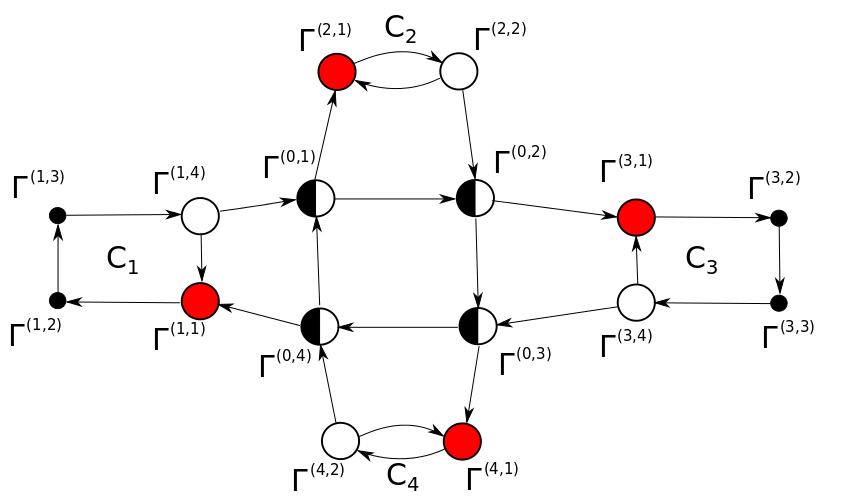
\includegraphics[scale=0.5]{GraphScheme3.png} 
\caption{Класс графов переходов. Незакрашенные вершины являются выходными вершинами, красным отмечены входные вершины, черным --- нейтральные, наполовину закрашенным вершинам соответствуют состояния продления}
\label{GraphScheme}
\end{figure}
%\subsection{Допустимые графы переходов состояний ОУ}

Рассмотрим введеные обозначения на примере Рис.~\ref{GraphScheme}. Примерами входных состояний являются $\ga{1,1} \in C_1^{\mathrm{I}}$ и $\ga{2,3} \in C_2^{\mathrm{I}}$, выходных состояний~--- $\ga{1,4} \in C_1^{\mathrm{O}}$ и $\ga{2,1} \in C_2^{\mathrm{O}}$, нейтральных состояний~--- $\ga{1,2}, \ga{1,3}, \ga{1,n_1} \in C_1^{\mathrm{N}}$ и $\ga{2,2} \in C_2^{\mathrm{N}}$. Состояния продления представлены на графе вершинами $\ga{0,1}$, $\ga{0,2}$, $\ga{0,3}$ и $\ga{0,4}$. Далее, отображение $h_1(\cdot)$ на графе задано таким образом, что оно переводит, например, выходное состояние $\ga{1,4}$ в число $1$~--- номер состояния продления $\ga{0,1}$, то есть $h_1(\ga{1,4})=1$. Аналогично $h_2(1)=2$, $h_2(2)=4$ и $h_2(3)=1$. Примером отображения $h_3(\cdot)$ является $h_3(2)=\ga{2,3}$.

Таким образом, смена состояний обслуживающего устройства задается соотношением:
\begin{equation}
h(\ga{k,r},x) = 
\begin{cases}
\ga{k,r\oplus_k 1},& \quad \text{ если } \ga{k,r}\in C_k\setminus C_k^{\mathrm{O}}\\
\ga{k,r\oplus_k 1},& \quad \text{ если } \ga{k,r}\in C_k^{\mathrm{O}} \text{ и } x>L\\
\ga{k,h_1(\ga{k,r})},& \quad \text{ если } \ga{k,r}\in C_k^{\mathrm{O}} \text{ и } x\leqslant L\\
\ga{0,h_2(r)},& \quad \text{ если } k=0 \text{ и } x\leqslant L\\
h_3(r),& \quad \text{ если } k=0 \text{ и } x > L
\end{cases}
\label{hLaw}
\end{equation}

Предполагается, что длительности обслуживания различных требований могут быть зависимыми и иметь различные законы распределения, поэтому вместо классического способа, состоящего в указании функции распределения длительности обслуживания произвольного требования, будут использованы потоки насыщения. Потоки насыщения $\Pi^{\mathrm{\text{нас}}}_j$, $j \in \{1,2,3,4\}$, определяются как виртуальные выходные потоки при 
условии максимального использования ресурсов обслуживающего устройства, а для $j\in \{1, 2, 3\}$ еще и при условии максимальной загрузки соответствующих очередей. Пусть ${}^1\G=\G^{\mathrm{\Rmnum{1}}} \cup \G^{\mathrm{\Rmnum{3}}}$, 
${}^2\G=\G^{\mathrm{\Rmnum{1}}} \cup \G^{\mathrm{\Rmnum{2}}}$,
${}^3\G=\G^{\mathrm{\Rmnum{3}}} \cup \G^{\mathrm{\Rmnum{4}}}$. 
Тогда поток насыщения $\Pi^{\mathrm{\text{нас}}}_j$, $j\in \{1,2,3\}$, будет содержать неслучайное число $\ell_{k,r,j}$ требований, обслуженных в течение времени $\Tt{k,r}$, если $\ga{k,r} \in~^j\G$, и будет содержать $0$ требований в противном случае: $\ga{k,r} \notin ~^j\G$. Пусть $Z_+$~--- множество целых неотрицательных чисел. Тогда, при условии, что в очереди $O_4$ находится $x \in Z_+$ требований, поток насыщения $\Pi^{\mathrm{\text{нас}}}_4$ определим как поток, содержащий все $x$ требований.
%\subsection{Пример: тандем из двух перекрестков} 
Наконец, при состоянии обслуживающего устройства $\ga{k,r}$ каждое требование из очереди $O_4$ с вероятностью $p_{k,r}$ и независимо от других завершает обслуживание и отправляется в очередь $O_2$ потока~$\Pi_2$. С вероятностью $1-p_{k,r}$ требование очереди $O_4$ остается в ней до следующего такта. На следующем такте процесс повторяется.

В качестве наглядной физической интерпретации можно привести тандем из двух перекрестков (рис. \ref{crossroads}).
\begin{figure}[h]
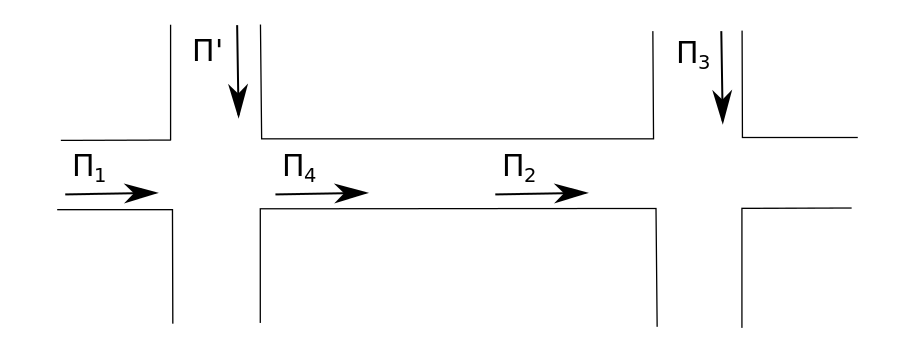
\includegraphics[scale=0.5]{Crossroads.png} 
\caption{Пример: тандем перекрестков}
\label{crossroads}
\end{figure}
В качестве потоков требований, формируемых внешней средой, выступают потоки прибывающих на перекрестки машин: конфликтные потоки $\Pi_1$, $\Pi_5$ на первом перекрестке, а также поток $\Pi_3$ на втором. Каждая машина из потока $\Pi_1$, проезжая первый перекресток, становится в очередь $O_4$ потока $\Pi_4$ и затем с некой вероятностью ($p_{k,r}$ для состояния $\ga{k,r}$ обслуживающего устройства) доезжает до следующего перекрестка, или же не успевает это сделать и остается в очереди $O_4$ до следующего такта обслуживания. В случае, если машина из очереди $O_4$ успевает доехать до второго перекрестка, она становится в очередь $O_2$ и ждет своей очереди для его прохождения.

Предполагается, что светофор на первом перекрестке имеет лишь два состояния $\{g_{1,1},g_{1,2}\}$: в состоянии $g_{1,1}$ машины потока $\Pi_1$ пропускаются фиксированное количество времени $\widetilde T^{(1,1)}$ (<<зеленый>> свет для $\Pi_1$); в состоянии $g_{1,2}$ --- простаивают в течение времени $\widetilde T^{(1,2)}$ (<<красный>> свет для $\Pi_1$). Светофор на втором перекрестке обслуживает по алгоритму с продлением: дополнительно к состоянию обслуживания потока $\Pi_1$ (состояние $g_{2,1}$), также имеется два состояния обслуживания потока $\Pi_2$ (состояния $\{g_{2,2},g_{2,3}\}$). Первое из них включается всегда после завершения обслуживания потока $\Pi_3$, а второе включается, если после очередного такта обслуживания потока $\Pi_2$ длина очереди $O_3$ не превосходит уровня $L$.
Длительности пребывания светофора на втором перекрестке в каждом из состояний суть $\widetilde T^{(2,1)}$, $\widetilde T^{(2,2)}$ и $\widetilde T^{(2,3)}$.

% В этом особом состоянии продления светофор продолжает пропускать машины потока $\Pi_3$ в течение фиксированного количества времени, вообще говоря, отличного от времени обслуживания в штатном режиме. В режим продления светофор переходит в случае, когда штатное обслуживание требований потока $\Pi_3$ закончено, однако количество требований (машин) в очереди $O_3$ еще превышает некий заданный порог $g$. В случае, если по истечении периода продления в очереди $O_3$ еще будет находиться достаточное число требований (превышающее заданный порог $L$), светофор проводит столько тактов продления дополнительно, сколько будет нужно для снижения количества машин в очереди $O_3$ до порога $L$.
%
 
Рассматривая тандем из двух перекрестков как единую систему массового обслуживания и предполагая наблюдение за ней только в (дискретные) моменты переключения состояния хотя бы одного из светофоров, может быть показано, что количество различных состояний у полученной системы конечно. Действительно, положим, например, за состояние объединенной системы вектор $(g^{(1)},g^{(2)}, s, t)$, где $g^{(1)}\in \{g_{1,1},g_{1,2}\}$~--- состояние $1$--го перекрестка, $g^{(2)}\in \{g_{2,1},g_{2,2},g_{2,3}\}$~--- состояние $2$--го перекрестка, $s \in \{0, 1, 2\}$~--- номер последнего сменившего состояние перекрестка (принимает значение $0$ в случае, если сменили состояние оба перекрестка) и $t \in \{0, 1, 2, \ldots, T\}$~--- количество времени, оставшееся у продолжающего обслуживание с прошлого такта перекрестка (принимает значение $0$, если принимает значение $0$ величина $s$). Здесь $T$~--- максимальная длительность нахождения каждого из светофоров в одном состоянии. Тогда количество различных состояний не трудно посчитать и оно не будет превышать величины  $2\times 3 \times 3 \times T$.

В завершение построения примера отметим, что при прохождении перекрестков машины предполагаются движущимися только в прямом направлении, то есть перемешивания конфликтных потоков не допускается. Таким образом, поток $\Pi_5$ не представляет интереса для дальнейшего исследования системы и может быть отброшен и, следовательно, построенный пример целиком удовлетворяет структурной схеме на рис. \ref{SystemScheme}.

Теперь продемонстрируем на конкретном числовом примере выделение циклов и состояний продления. Пусть изменение состояний перекрестков и время пребывания (в секундах для определнности) в каждом из состояний задается графами на рис. \ref{SystemStates}.
\begin{figure}[h]
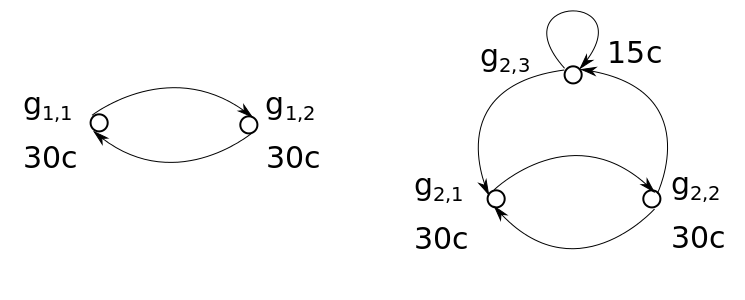
\includegraphics[scale=0.5]{SystemStates.png} 
\caption{Числовой пример тандема перекрестков. Левый граф соответствует первому перекрестку, правый~--- второму}
\label{SystemStates}
\end{figure}
За начальное состояние объединенной системы примем $\G_0=(g_{1,1},g_{2,1},0,0)$, то есть первый перекресток находится в состоянии $g_{1,1}$, второй~--- в состоянии $g_{2,1}$, и оба только начали свою работу в своем состоянии (этот факт моделируется равенствами $s=0$ и $t=0$). Следующая смена состояний случится у обоих перекрестков одновременно и приведет к следующему состоянию $(g_{1,2},g_{2,2}, 0, 0)$. Далее смена состояний произойдет также у первого и второго перекрестков, однако второй перекресток может перейти как в состояние $g_{2,1}$, так и в состояние продления $g_{2,3}$. Таким образом следущим состоянием тандема будет либо опять $(g_{1,1},g_{2,1},0,0)$, либо $(g_{1,1},g_{2,3},0,0)$. Продолжая рассуждения аналогичным образом, получим следущий список всех возможных состояний системы:
\begin{align*}
(g_{1,1},g_{2,1},0,0)&=\ga{1,1} ,& \quad (g_{1,2},g_{2,2},0,0)&=\ga{1,2} ,& \quad (g_{1,1},g_{2,3},0,0)&=\ga{0,1}, \\
(g_{1,1},g_{2,3},15,2)&=\ga{0,2} ,& \quad (g_{1,2},g_{2,3},0,0)&=\ga{0,3} ,& \quad (g_{1,2},g_{2,3},15,2)&=\ga{0,4}, \\
(g_{1,2},g_{2,1},15,2)&=\ga{4,1} ,& \quad (g_{1,1},g_{2,1},15,1)&=\ga{4,2} ,& \quad (g_{1,1},g_{2,2},15,2)&=\ga{4,3}, \\
(g_{1,2},g_{2,2},15,1)&=\ga{4,4} ,& \quad (g_{1,2},g_{2,3},15,2)&=\ga{0,5} ,& \quad (g_{1,2},g_{2,1},0,0)&=\ga{3,1}, \\
(g_{1,1},g_{2,2},0,0)&=\ga{3,2} ,& \quad (g_{1,1},g_{2,1},15,2)&=\ga{2,1} ,& \quad (g_{1,2},g_{2,1},15,1)&=\ga{2,2}, \\
(g_{1,2},g_{2,2},15,2)&=\ga{2,3} ,& \quad (g_{1,1},g_{2,2},15,1)&=\ga{2,4}. & &
\end{align*}
В соответсвии с приведенными выше обозначениями, множества $C_1$, $C_2$, $C_3$, $C_4$, а также множество состояний продления строятся однозначным образом. Множествами входных состояний будут $C_1^{\mathrm{I}}=\{\ga{1,1}\}$, $C_2^{\mathrm{I}}=\{\ga{2,1}\}$, $C_3^{\mathrm{I}}=\{\ga{3,1}\}$ и $C_4^{\mathrm{I}}=\{\ga{4,1}\}$. Множествами выходных состояний будут $C_1^{\mathrm{O}}=\{\ga{1,2}\}$, $C_2^{\mathrm{O}}=\{\ga{2,4}\}$, $C_3^{\mathrm{O}}=\{\ga{3,2}\}$ и $C_4^{\mathrm{O}}=\{\ga{4,4}\}$. Функции $h_1(\cdot)$, $h_2(\cdot)$ и $h_3(\cdot)$ задаются поточечно:
\begin{equation*}
h_1(\ga{1,2})=1, \quad h_1(\ga{2,4})=2, \quad h_1(\ga{3,2})=3, \quad h_1(\ga{4,4})=5,
\end{equation*}
\begin{equation*}
h_2(1)=2, \quad h_2(2)=3, \quad h_2(3)=4 \quad h_2(4)=1, \quad h_2(5)=1,
\end{equation*}
\begin{equation*}
h_3(1)=\ga{2,1}, \quad h_3(2)=\ga{3,1}, \quad h_3(3)=\ga{4,1} \quad h_3(4)=\ga{1,1}, \quad h_3(5)=\ga{1,1}.
\end{equation*}
Этим завершается построение числового примера.

\subsection{Представление рассматриваемой системы обслуживания в виде кибернетической управляющей системы}
Описанная в предыдущем разделе на содержательном уровне система массового обслуживания должна рассматриваться как кибернетическая управляющая система обслуживания (ссылка на федоткина, Зорина А.В. киевский сборник твмс). Схема управляющей системы приведена на рис. \ref{SystemScheme}. На схеме присутствуют следующие блоки: 1) внешняя среда с одним состоянием; 2) входные полюса первого типа~--- входные потоки $\Pi_1$, $\Pi_2$, $\Pi_3$, $\Pi_4$; 3) входные полюса второго типа~--- потоки насыщения $\Pi_1^{\mathrm{\text{нас}}}$, $\Pi_2^{\mathrm{\text{нас}}}$, $\Pi_3^{\mathrm{\text{нас}}}$, $\Pi_4^{\mathrm{\text{нас}}}$; 4) внешняя память~--- очереди $O_1$, $O_2$, $O_3$, $O_4$; 5) устройство по переработки информации внешней памяти~--- устройства по поддержанию дисциплины очереди $\delta_1$, $\delta_2$, $\delta_3$, $\delta_4$; 6) внутренняя память обслуживающего устройства~--- обслуживающее устройство (ОУ); 7) устройство по переработке информации во внутренней памяти~--- граф смены состояний; 8) выходные полюса $\Pi_1^{\mathrm{\text{вых}}}$, $\Pi_2^{\mathrm{\text{вых}}}$, $\Pi_3^{\mathrm{\text{вых}}}$, $\Pi_4^{\mathrm{\text{вых}}}$. Координатой блока является номер этого блока на схеме. 

Для задания информации блоков введем следующие величины и элементы, а также укажем множества их возможных значений. В качестве дискретной временной шкалы выберем последовательность $\tau_0=0$, $\tau_1$, $\tau_2$, $\ldots$ моментов смены состояний обслуживающего устройства. Обозначим $\G_i$ из множества $\G$ состояние обслуживающего устройства в течение времени $\left(\tau_{i-1};\tau_i\right]$, количество $\vk_{j,i} \in Z_+ $ требований в очереди $O_j$ в момент времени $\tau_i$, количество $\eta_{j,i} \in Z_+$ требований, поступивших в очередь $O_j$ по потоку $\Pi_j$ в течение времени $\left(\tau_{i};\tau_{i+1}\right]$, количество $\xi_{j,i} \in Z_+$ требований по потоку насыщения $\Pi^{\mathrm{\text{нас}}}_j$ в течение времени $\left(\tau_{i};\tau_{i+1}\right]$, количество $\overline{\xi}_{j,i}\in Z_+$ реально обслуженных требований по потоку $\Pi_j$ в течение времени $\left(\tau_{i};\tau_{i+1}\right]$, $j\in \{1,2,3,4\}$.

Закон изменения состояния обслуживающего устройства будем предполагать заданным соотношением 
\begin{equation}
\G_{i+1}=h(\G_i,\vk_{3,i}),
\label{gammaFunc}
\end{equation}
где отображение $h(\cdot,\cdot)$ определено в \eqref{hLaw}.
Для определения длительности $T_{i+1}$ состояния обслуживающего устройства в течение времени $\left(\tau_{i};\tau_{i+1}\right]$, удобно ввести функцию $h_T(\cdot,\cdot)$:
\begin{equation*}
T_{i+1}=h_T(\G_i,\vk_{3,i})= \Tt{k,r},\quad  \text{ где } \ga{k,r}=\G_{i+1}=h(\G_i,\vk_{3,i}).
%\label{timeLaw}
\end{equation*}
Функциональная зависимость
\begin{equation}
\overline{\xi}_{j,i}=\min\{\vk_{j,i}+\eta_{j,i},\xi_{j,i}\}, \quad j\in \{1,2,3\},
\label{saturationEq}
\end{equation}
между величиной $\overline{\xi}_{j,i}$ и величинами $\vk_{j,i}$, $\eta_{j,i}$, $\xi_{j,i}$ реализует стратегию механизма обслуживания требований. Далее, поскольку 
\begin{equation*}
\vk_{j,i+1}=\vk_{j,i}+\eta_{j,i}-\overline{\xi}_{j,i}, \quad  j\in \{1,2,3\},
\end{equation*}
то из \eqref{saturationEq} следует соотношение
\begin{equation}
\vk_{j,i+1}=\max\{{0,\vk_{j,i}+\eta_{j,i}-\xi_{j,i}}\}, \quad j\in \{1,2,3\}.
\label{queuesFunc}
\end{equation}
Из формулировки поставленной задачи (см. также структурную схему \eqref{SystemScheme}) следуют соотношения для потока $\Pi_4$:
\begin{equation}
\eta_{4,i} = \min\{\xi_{1,i}, \vk_{1,i}+\eta_{1,i}\}, \quad \vk_{4,i+1}=\vk_{4,i}+\eta_{4,i}-\eta_{2,i}, \quad \xi_{4,i} = \vk_{4,i}.
\label{FourthFunc}
\end{equation}

Нелокальное описание входных потоков и потоков насыщения состоит в указании некоторых свойств условных распределений выделенных дискретных компонент $\eta_i=(\eta_{1,i},\eta_{2,i}, \eta_{3,i}, \eta_{4,i})$ и $\xi_i=(\xi_{1,i}, \xi_{2,i}, \xi_{3,i}, \xi_{4,i})$ маркированных точечных процессов \linebreak $\{(\tau_i, \nu_i, \eta_i); i\geqslant 0\}$ и $\{(\tau_i, \nu_i, \xi_i); i\geqslant 0\}$ при фиксированных значениях метки $\nu_i = (\Gamma_i,(\vk_{1,i},\vk_{2,i},\vk_{3,i},\vk_{4,i}))$. 
Введем функции $\vp_1(\cdot,\cdot)$, $\vp_3(\cdot,\cdot)$ из разложений 
\begin{equation*}
\sum_{x=0}^{\infty} z^x\vp_j(x,t) = \exp\{\la_j t (f_j(z)-1)\},
\end{equation*}
где $f_j(z)$ определены в \eqref{GeneratingFunc}, $j \in \{1,3\}$. Функция $\vp_j(x,t)$ есть вероятность поступления $x=0$, $1$, $\ldots$ требований по потоку $\Pi_j$ за время $t \geqslant 0$. Функция $\psi(\cdot,\cdot,\cdot)$ задается формулой
\begin{equation*}
\psi(k;x,u)=C_x^k u^k (1-u)^{x-k}
\end{equation*}
и по своему смыслу есть вероятность поступления $k$ требований по потоку $\Pi_2$, при условии, что очередь $O_4$ содержит $x$ требований и обслуживающее устройство находится в состоянии $\ga{k,r}$, так что $u=p_{k,r}$.


При фиксированном значении метки $\nu_i=(\ga{k,r},(x_1, x_2, x_3, x_4))$ вероятность одновременного выполнения равенств $\eta_{1,i}=a_1$, $\eta_{2,i}=a_2$, $\eta_{3,i}=a_3$, $\eta_{4,i}=a_4$ есть 
\begin{equation}
\vp_1(a_1,h_T(\ga{{k},{r}},x_3)) \times \psi(a_2,x_2, p_{\tilde{k},\tilde{r}}) \times \vp_1(a_3,h_T(\ga{{k},{r}},x_3))
\times \delta_{a_4,\min{\{\tilde{\ell}(\tilde{k},\tilde{r},1), x_1+a_1}\}},
\label{conditionProbOne}
\end{equation}
где $0\leqslant a_2\leqslant x_2$, $a_1$, $a_3$, $a_4$ $\in Z_+$, $\ga{\tilde{k},\tilde{r}}=h(\ga{k,r},x_3)$,  $\delta_{i,j}$ есть символ Кронекера
\begin{equation*}
\delta_{i,j}=\begin{cases} 1, \quad \text{ если }i=j\\0, \quad \text{ иначе}
\end{cases},
\end{equation*}
и
\begin{equation*}
\widetilde{\ell}(k,r,j)=\begin{cases}\ell_{k,r,j},& \quad \text{если } \ga{k,r} \in {}^j\G\\0,& \quad \text{иначе}  \end{cases},
\quad j\in \{1, 2, 3\}.
\end{equation*}
Поскольку для $j\in \{1, 2, 3\}$ поток насыщения $\Pi_j^{\mathrm{\text{нас}}}$ содержит ненулевое количество требований только в случае обслуживания потока $\Pi_j$, то вероятность того, что $\xi_{j,i} = 0$ равна $1$ в случае $h(\ga{k,r},x_3)\notin {}^j\G$. По тем же причинам вероятность того, что $\xi_{j,i} = \ell_{\tilde{k},\tilde{r},j}$ равна $1$, если $\ga{\tilde{k},\tilde{r}}=h(\ga{k,r},x_3)\in {}^j\G$. Таким образом, вероятность одновременного выполнения равенств $\xi_{1,i}=b_1$, $\xi_{2,i}=b_2$, $\xi_{3,i}=b_3$, $\xi_{4,i}=b_4$ при фиксированном значении метки $\nu_i=(\ga{k,r},(x_1, x_2, x_3, x_4))$ есть
\begin{equation}
\delta_{b_1,\tilde{\ell}(\tilde{k},\tilde{r},1)} \times \delta_{b_2,\tilde{\ell}(\tilde{k},\tilde{r},2)} \times 
\delta_{b_3,\tilde{\ell}(\tilde{k},\tilde{r},3)} \times \delta_{b_4,x_4}.
\label{conditionProbTwo}
\end{equation}

%где $0\leqslant a \leqslant x_4$, $b,x,x_3,x_4 \in Z_+$, $\gamma \in \G$.

%$\vp_j(a,h_T(\ga{k,r},x))$, $j=1$, $3$.  
%\begin{equation*}
%\begin{aligned}
%f_{\xi_j | \G,\vk_3} (\gamma,x_3) &= \ell_{k,r,j},\text{ где }  h(\gamma,x)=\ga{k,r}\in {}^j\G \text{ и } j\in\brrr{1,2,3}\\
%f_{\eta_4| \xi_1, \eta_1, \vk_1} (a,b,x) &= \begin{cases} a,\quad &\text{если }x+b\geq a \\  x+b,\quad &\text{если }x+b<a \end{cases},
%\end{aligned}
%\end{equation*}
%и
%\begin{equation*}
%\begin{aligned}
%P_{\eta_1|\G,\vk_3}(a,\gamma,x) &= \vp_1(a,h_T(\gamma,x))
%\end{aligned}
%\end{equation*}

%\begin{equation}
%P_{\eta_2|\G,\vk_3,\vk_4} (a,\gamma,x_3,x_4) &= \begin{cases} \binom{x_4}{a} p_{k,r}^a(1-p_{k,r})^{x_4-a}, \quad &\text{если } h(\gamma,x_3)=\ga{k,r} \\ 0, \quad &\text{иначе}\end{cases}, \\
%\end{equation}

%, где $\vk_i=(\vk_{1,i}, \vk_{2,i}, \vk_{3,i}, \vk_{4,i})$.
%
%\item количество $\vk_{j,i} \in Z_+ $ требований в очереди $O_j$ в момент времени $\tau_i$;
%\item состояние обслуживающего устройства $\G_i\in \G = \brrr{\G^{(1)},\G^{(2)}, \ldots, \G^{(n)}}$ в течение времени $\left(\tau_{i-1};\tau_i\right]$;
%\item количество $\eta_{j,i}$ требований, поступивших в очередь $O_j$ по потоку $\Pi_j$ в течение времени $\left(\tau_{i};\tau_{i+1}\right]$;
%\item количество $\xi_{j,i}$ требований по потоку насыщения $\Pi^{\mathrm{sat}}_j$ в течение времени $\left(\tau_{i};\tau_{i+1}\right]$;
%\item количество $\overline{\xi}_{j,i}$ реально обслуженных требований по потоку $\Pi_j$ в течение времени $\left(\tau_{i};\tau_{i+1}\right]$.


Построим теперь 	вероятностное пространство $(\Omega, {\cal F}, \Pr(\cdot))$, чтобы можно было рассматривать введеные величины как случайные величины на этом пространстве. А именно, докажем следующую теорему.
\begin{theorem}
Пусть $\gamma_0=\ga{k,r} \in \G$ и $x_0=(x_{1,0},x_{2,0}, x_{3,0},x_{4,0})$ фиксированы.
Тогда существует вероятностное пространство $(\Omega, {\cal F}, \Pr(\cdot))$ и заданные на нем случайные величины $\eta_{j,i}=\eta_{j,i}(\omega)$, $\xi_{j,i}=\xi_{j,i}(\omega)$, $\overline{\xi}_{j,i}=\overline{\xi}_{j,i}(\omega)$,  $\vk_{j,i}=\vk_{j,i}(\omega)$, $\G_i=\G_i(\omega)$, $i\geqslant 0$, $j\in \{1, 2, 3, 4\}$, такие, что $\G_0(\omega) = \gamma_0$ и $\vk_0(\omega)=x_0$, выполняются соотношения \eqref{gammaFunc}, \eqref{queuesFunc}, \eqref{FourthFunc} и для любых $a_j, b_j \in Z_+$ $x \in Z_+^4$ верно равенство
\ml
{
\Pr \{\omega \colon \eta_{1,i}=a_1, \eta_{2,i}=a_2, \eta_{3,i}=a_3, \eta_{4,i}=a_4; \xi_{1,i}=b_1, \xi_{2,i}=b_2, \xi_{3,i}=b_3, \xi_{4,i}=b_4|\\
| \G_i=\ga{k,r},\vk_{i}=x\} = \Pr \{\omega \colon \eta_{1,i}=a_1, \eta_{2,i}=a_2, \eta_{3,i}=a_3, \eta_{4,i}=a_4 | \G_i=\ga{k,r},\vk_{i}=x\}
\times \\
\times \Pr \{\omega \colon \xi_{1,i}=b_1, \xi_{2,i}=b_2, \xi_{3,i}=b_3, \xi_{4,i}=b_4| \G_i=\ga{k,r},\vk_{i}=x\}
}
причем первый и второй множитель находятся из соотношений \eqref{conditionProbOne} и \eqref{conditionProbTwo} соответственно.
%для событий 
%\begin{gather}
%\begin{aligned}
%A_i(k;r;x_1;x_2;x_3;x_4) &= \{\omega \colon\G_i=\ga{k,r},\vk_{3,i}=x_3\}\cap\\ 
%& \quad \cap \{\omega \colon \vk_{1,i}=x_1,\vk_{2,i}=x_2,\vk_{4,i}=x_4\},
%\end{aligned}\\
%\begin{aligned}
%B_i(b_1;b_2;b_3;y_1;y_2;y_3) &= \{\omega \colon \eta_{1,i}=b_1, \eta_{2,i}=b_2, \eta_{3,i}=b_3\} \cap \\
%&\quad \cap \{\omega \colon \xi_{1,i}=y_1,\xi_{2,i}=y_2,\xi_{3,i}=y_3\}
%\end{aligned}
%\end{gather}
%значение вероятности
%\begin{equation*}
%\Pr \Bigl(B_i(b_1;b_2;b_3;y_1;y_2;y_3)\Big|\bigcap_{t=0}^{i} A_t(k_t;r_t;x_{1,t};x_{2,t};x_{3,t};x_{4,t})\Bigr)
%\end{equation*}
%задается формулой \eqref{conditionProb}.
\label{myTheorem}
\end{theorem}
\begin{proof}
В соответствии с теоремой Ионеску Тулчи (ссылка) для доказательства достаточно задать на $(\Omega_0, {\cal F}_0)$ вероятностную меру $P_0(\cdot)$ и далее, считая для $0 < i \leqslant n$ и каждого набора элементарных исходов $(\omega_0, \omega_1, \ldots, \omega_{i-1})$ заданной на $(\Omega_i, {\cal F}_i)$ вероятностную меру $P(\omega_0,\omega_1,\ldots, \omega_{i-1},\cdot)$, задать на $(\Omega_{n+1}, {\cal F}_{n+1})$ меру $P(\omega_0,\omega_1,\ldots, \omega_{n},\cdot)$, причем для любого множества $B\in {\cal F}_i$ функции $P(\omega_0,\omega_1,\ldots, \omega_{i-1},B)$
должны быть измеримыми функциями от $(\omega_0, \omega_1, \ldots, \omega_{i-1})$. Тогда для $\Omega=\prod\limits_{i=0}^{\infty}\Omega_i$ и ${\cal F}=\bigotimes\limits_{i=0}^{\infty} {\cal F}_i$ на $(\Omega,{\cal F})$ будет существовать единственная вероятностная мера $\Pr(\cdot)$ такая, что для любого $i \geqslant 0$
\begin{equation}
\Pr\{\omega \colon \omega_0 \in A_0, \omega_1 \in A_1, \ldots, \omega_i\in A_i\} = P_i(A_0 \times A_1 \times \ldots \times A_i),
\label{ProbabilitiesGeneral}
\end{equation}
где 
\begin{equation}
 P_i(A_0 \times A_1 \times \ldots \times A_i) = \int_{A_0} P_0(d \omega_0) \int_{A_1} P(\omega_0,d \omega_1) \ldots \int_{A_i} P(\omega_0, \omega_1, \ldots, \omega_{i-1}, d \omega_i),
\label{ProbabilitiesGeneralOne}
\end{equation}
$i\geqslant 0$, $A_i\in {\cal F}_i$. 
%Более того, наряду с вероятностной мерой $\Pr(\cdot)$ также будет существовать случайная последовательность $X=(X_0(\omega), X_1(\omega), \ldots)$ такая, что
%\begin{equation}
%\Pr\{\omega \colon X_0(\omega) \in A_0, X_1(\omega)\in A_1, \ldots, X_i(\omega)\in A_i\} = P_i(A_0\times A_1 \times \ldots, \times A_i),
%\label{ProbabilitiesGeneralTwo}
%\end{equation}
%где $i\geqslant 0$, $A_i\in {\cal F}_i$.

Итак, за описание элементарного исхода $\omega_i \in \Omega_i$ для произвольного $i \geqslant 0$ примем набор $\omega_i=(\omega_{1,i},\omega_{2,i},\omega_{3,i})$, $\omega_{j,i}\in Z_+$. Таким образом, $\Omega_i=Z_+^3$ и в качестве $\sigma$-алгебры ${\cal F}_i$ возьмем множество всех подмножеств $\Omega_i$: ${\cal F}_i=2^{\Omega_i}$. Пусть $\ga{\widetilde{k},\widetilde{r}}=h(\ga{k,r},x_{3,0})$. Тогда  поскольку множество $\Omega_0$ счетно, определим вероятностную меру $P_0(\cdot)$ на измеримом пространстве $(\Omega_0,{\cal F}_0)$ ее значениями на одноточечных множествах:
\begin{equation}
P_0(\{(a_1,a_2,a_3)\})=\vp_1(a_1,h_T(\ga{k,r})) \times \psi(a_2,x_{2,0}, p_{\tilde{k},\tilde{r}}) \times \vp_1(a_1,h_T(\ga{k,r})).
% \times \delta_{a_4,\min{\{\widetilde{\ell}_{\widetilde{k},\widetilde{r},1}, x_{1,0}+a_1}\}},
\label{probabilitiesOne}
\end{equation}

Определим величины
\begin{equation}
\G_0=\gamma_0, \quad \vk_{j,0}=x_{j,0}, \quad \xi_{j,0}(\omega_0)=\widetilde{l}(\tilde{k},\tilde{r},j),
\label{startRekOne}
\end{equation}
\begin{equation}
\eta_{j,0}=\omega_{j,0}, \quad \eta_{4,0}=\min\{\xi_{1,0}, x_{1,0}+\eta_{1,0}\}, \quad \xi_{4,0}=x_{4,0}.
\label{startRekTwo}
\end{equation}
где $j\in \{1,2,3\}$.
Теперь, предполагая заданными на $(\Omega_i, {\cal F}_i)$ вероятностные меры $P(\omega_0, \omega_1, \ldots, \omega_{i-1},\cdot)$, заданными величины $\G_i$, $\vk_{j,i}$, $\xi_{j,i}$, $\eta_{j,i}$, $i\in \{0,1,\ldots,n\}$, $j\in \{1, 2, 3, 4\}$ и фиксируя набор $(\omega_0, \omega_1, \ldots, \omega_{n})$, определим на $(\Omega_{n+1}, {\cal F}_{n+1})$ меру $P(\omega_0, \omega_1, \ldots, \omega_n,\cdot)$. Пусть
\begin{equation}
\G_{n+1}=\ga{k^*,r^*}=h(\G_{n},\vk_{3,n}), \quad \vk_{j,n+1}=\max\{ 0,\vk_{j,n}+\eta_{j,n} -\xi_{j,n}\},
%\label{functionsTwo}
\label{NextRekOne}
\end{equation}
\begin{equation}
\vk_{4,n+1}=\vk_{4,n}+\eta_{4,n}-\eta_{2,n}, \quad \xi_{j,n+1}=\widetilde{l}(k^*,r^*,j),
\label{NextRekTwo}
\end{equation}
\begin{equation}
\eta_{j,n+1}=\omega_{j,n+1}, \quad \eta_{4,n+1}=\min\{\xi_{1,n+1}, \vk_{1,n+1}+\eta_{1,n+1}\}, \quad \xi_{4,n+1}=\vk_{4,n+1},
\label{NextRekThree}
\end{equation}
для $j\in \{1, 2, 3\}$.
%\begin{equation}
%\begin{aligned}
%\xi_{j,i}(\omega_0,\omega_1,\ldots,\omega_i)&=f_{\xi_j | \G,\vk_3} (\G_i(\omega_0,\omega_1,\ldots,\omega_i),x_{3,i}(\omega_0,\omega_1,\ldots,\omega_i)),\\
%\eta_{j,i}(\omega_0,\omega_1,\ldots,\omega_i)&=\eta_{j,i}(\omega_i)=\eta_{j,i}(\omega_{1,i},\omega_{2,i},\omega_{3,i})=\omega_{j,i}, \\
%\eta_{4,i}(\omega_0,\omega_1,\ldots,\omega_i)&=f_{\eta_4| \xi_1, \eta_1, \vk_1} (\xi_{1,i}(\omega_0,\omega_1,\ldots,\omega_i),\eta_{1,i}(\omega_i),\vk_{1,i}(\omega_0,\omega_1,\ldots,\omega_i)),\\
%\overline{\xi}_{4,0}(\omega_0,\omega_1,\ldots,\omega_i)&=\eta_{2,0}(\omega_i)
%\end{aligned}
%\label{functionsThree}
%\end{equation}
%на пространствах $(\Omega_{i+1}, {\cal F}_{i+1},P_{i+1}(\omega_0, \omega_1, \ldots, \omega_{i},\cdot))$, $i\in \{0,1,\ldots,n-1\}$, $j\in \{1,2,3\}$ (которые являются константами относительно рассматриваемых пространств), и случайные величины 
%
%на пространствах  $(\Omega_{i}, {\cal F}_{i},P_{i}(\omega_0, \omega_1, \ldots, \omega_{i-1},\cdot))$, $i\in \{0,1,\ldots,n\}$, $j\in \{1,2,3\}$, построим меру $P_{n+1}(\omega_0, \omega_1, \ldots, \omega_{n},\cdot)$:
Тогда
\ml
{
P(\omega_0,\omega_1,\ldots,\omega_n,\{\omega_{n+1} \colon \omega_{1,n+1}=a_1, \omega_{2,n+1}=a_2, \omega_{3,n+1}=a_3\}) = \\
= \vp_1(a_1,h_T(\G_n,x_{3,n})) \times \psi(a_2,x_{2,n}, p_{k^*,r^*}) \times \vp_1(a_3,h_T(\G_n,x_{3,n})).
\label{probabilitiesTwo}
}
%\ml
%{
%P_{n+1}(\omega_0,\omega_1,\ldots,\omega_n,\{\omega_{n+1} = (\eta_{1,n+1},\eta_{2,n+1},\eta_{3,n+1})\colon \eta_{1,n+1}=a_1, \eta_{2,n+1}=a_2, \eta_{3,n+1}=a_3\}) = \\
%=P_{\eta_1|\G,\vk_3}(a_1,\G_{n+1}(\omega_0,\omega_1,\ldots,\omega_i),\vk_{3,n+1}(\omega_0,\omega_1,\ldots,\omega_{i}))\times\\
%\times P_{\eta_2|\G,\vk_3,\vk_4} (a_2,\G_{n+1}(\omega_0,\omega_1,\ldots,\omega_n),\vk_{4,n+1}(\omega_0,\omega_1,\ldots,\omega_{n})) \times\\
%\times P_{\eta_3|\G,\vk_3}(a_3,\G_{n+1}(\omega_0,\omega_1,\ldots,\omega_i),\vk_{3,n+1}(\omega_0,\omega_1,\ldots,\omega_{i})).
%\label{probabilitiesTwo}
%}
Вероятностное пространство $(\Omega,{\cal F},\Pr(\cdot))$ построено. 

Теперь докажем, что введеные с помощью \eqref{startRekOne}~--~\eqref{NextRekThree} случайные элементы $\G_i(\omega)$ и случайные величины $\vk_{j,i}(\omega)$, $\eta_{j,i}(\omega)$, $\xi_{j,i}$, $i \geqslant 0$, $j \in \{1, 2, 3, 4\}$ удовлетворяют условиям теоремы. Из построения следует, что случайные элементы $\G_i$ удовлетворяют \eqref{gammaFunc}, а случайные величины $\vk_{j,i}$ удовлетворяют \eqref{queuesFunc} и \eqref{FourthFunc}, $j\in \{1, 2, 3, 4\}$. Что касается $\xi_{j,i}$ и $\eta_{j,i}$, то для них найдем явное выражение для условной вероятности $\Pr\{\omega\colon \eta_{j,i}(\omega)=a_j, j\in\{1,2,3,4\} | \G_i(\omega)=\ga{k_1,r_1}, \vk_{i}(\omega)=x\}$. Пусть $\ga{k^*_1,r^*_1}=h(\ga{k_1,r_1},x)$. Учитывая \eqref{NextRekTwo} и \eqref{NextRekThree}, распишем по определению условной вероятности:
\mll
{
\Pr\{\omega \colon \omega_{j,i}=a_j, j\in \{1, 2, 3\}, a_4=\min\{\tilde{\ell}(k^*_1,r^*_1,1),x_{1} + a_1\}; \G_i(\omega_0,\omega_1,\ldots, \omega_{i-1})=\ga{k_1,r_1},\\
 \vk_i(\omega_0,\omega_1,\ldots, \omega_{i-1})=x\} / \Pr\{\omega \colon \G_i(\omega_0,\omega_1,\ldots, \omega_{i-1})=\ga{k_1,r_1}, \vk_i(\omega_0,\omega_1,\ldots, \omega_{i-1})=x\} = \\
 = \delta_{a_4, \min\{\tilde{\ell}(k^*,r^*,1),x_{1} + a_1\}} \times \Pr\{\omega \colon \omega_{j,i}=a_j, j\in \{1, 2, 3\}; \G_i(\omega_0,\omega_1,\ldots, \omega_{i-1})=\ga{k_1,r_1},\\
 \vk_i(\omega_0,\omega_1,\ldots, \omega_{i-1})=x\} / \Pr\{\omega \colon \G_i(\omega_0,\omega_1,\ldots, \omega_{i-1})=\ga{k_1,r_1}, \vk_i(\omega_0,\omega_1,\ldots, \omega_{i-1})=x\}.
}
Далее из \eqref{ProbabilitiesGeneral} и \eqref{ProbabilitiesGeneralOne} получим выражение для знаменателя последней дроби
\mll
{
\Pr\{\omega \colon \G_i(\omega_0,\omega_1,\ldots, \omega_{i-1})=\ga{k_1,r_1}, \vk_i(\omega_0,\omega_1,\ldots, \omega_{i-1})=x\} = \\
= \sum_{\substack{\omega_0, \omega_1,\ldots \omega_{i-1} \colon \\ \G_i=\ga{k_1,r_1}, \vk_i=x}} P_0(\omega_0)\times P(\omega_0;\{\omega_1\})\times\ldots\times P(\omega_0,\omega_1,\ldots, \omega_{i-2};\{\omega_{i-1}\})
}
и числителя
\mll
{
\Pr\{\omega \colon \omega_{j,i}=a_j, j\in \{1, 2, 3\}; \G_i(\omega_0,\omega_1,\ldots, \omega_{i-1})=\ga{k_1,r_1}, \vk_i(\omega_0,\omega_1,\ldots, \omega_{i-1})=x\} = \\
= \sum_{\substack{\omega_0, \omega_1,\ldots \omega_{i-1} \colon \\ \G_i=\ga{k_1,r_1}, \vk_i=x} } P_0(\omega_0)\times P(\omega_0;\{\omega_1\})\times\ldots\times P(\omega_0,\omega_1,\ldots, \omega_{i-2};\{\omega_{i-1}\})\times \\ 
\times P(\omega_0,\omega_1,\ldots, \omega_{i-1};\{\omega_{i}\})= \vp_1(a_1,h_T(\ga{k_1,r_1},x_{3})) \times \psi(a_2,x_{2}, p_{k^*_1,r^*_1}) \times \\ \times \vp_1(a_3,h_T(\ga{k_1,r_1},x_{3}))\sum_{\substack{\omega_0, \omega_1,\ldots \omega_{i-1} \colon \\ \G_i=\ga{k_1,r_1}, \vk_i=x} } P_0(\omega_0)\times P(\omega_0;\{\omega_1\})\times\ldots
\times P(\omega_0,\omega_1,\ldots, \omega_{i-2};\{\omega_{i-1}\})
}
После сокращения одинаковых сумм получим:
\mll
{
\Pr\{\omega\colon \eta_{j,i}(\omega)=a_j, j\in\{1,2,3,4\} | \G_i(\omega)=\ga{k_1,r_1}, \vk_{i}(\omega)=x\}=\\
=  \vp_1(a_1,h_T(\ga{k_1,r_1},x_{3})) \times \psi(a_2,x_{2}, p_{k^*_1,r^*_1}) \times \vp_1(a_3,h_T(\ga{k_1,r_1},x_{3})) \times \delta_{a_4, \min\{\tilde{\ell}(k^*_1,r^*_1,1),x_{1} + a_1\}},
}
что в точности совпадает с \eqref{conditionProbOne}. Аналогичным образом вероятность одновременного выполнения равенств $\xi_{1,i}=b_1$, $\xi_{2,i}=b_2$, $\xi_{3,i}=b_3$, $\xi_{4,i}=b_4$ при условии $\G_i(\omega)=\ga{k_1,r_1}$ и $\vk_{i}(\omega)=x$ совпадает с \eqref{conditionProbTwo}.
\end{proof}
%\ml
%{
%
%}

Таким образом, кибернетический подход позволил построить математическую модель управляющей системы обслуживания в виде последовательности случайных величин и случайных элементов, конструктивно заданных на некотором вероятностном пространстве. Выберем для исследования состояния обслуживающего устройства и длины всех очередей.

\subsection[Марковское свойство последовательности $\boldsymbol{\Mark}$]%
{Марковское свойство последовательности \\ $\boldsymbol{\Mark}$}

Теперь перейдем к вопросу о марковости последовательности $\Mark$. Введем следующие события:
\begin{align}
A_i(k;r;x_1;x_2;x_3;x_4) &= \{\G_i=\ga{k,r},\vk_{3,i}=x_3\}\bigcap \{\vk_{1,i}=x_1,\vk_{2,i}=x_2,\vk_{4,i}=x_4\},\\
B_i(b_1;b_2;b_3;y_1;y_2;y_3) &= \{\eta_{1,i}=b_1, \eta_{2,i}=b_2,\eta_{3,i}=b_3\} \bigcap \{\xi_{1,i}=y_1,\xi_{2,i}=y_2,\xi_{3,i}=y_3\}
\end{align}
Из теоремы \eqref{myTheorem} следует, что 
\ml
{
\P{B_i(b_1;b_2;b_3;y_1;y_2;y_3)}{\bigcap_{t=0}^{i} A_t(k_t;r_t;x_{1,t};x_{2,t};x_{3,t};x_{4,t})} = \\
\P{B_i(b_1;b_2;b_3;y_1;y_2;y_3)}{A_i(k_i;r_i;x_{1,i};x_{2,i};x_{3,i};x_{4,i})}
%= \P{\eta_{1,i}=b_1, \eta_{3,i}=b_3, \xi_{1,i}=y_1, \xi_{2,i}=y_2, \xi_{3,i}=y_3;\overline{\xi}_{4,i}=y_4}{\G_i=\ga{k_i,r_i},\vk_{3,i}=x_{3,i}}=\\
%= \P{\eta_{1,i}=b_1}{\G_i=\ga{k_i,r_i},\vk_{3,i}=x_{3,i}} \times
%\P{\eta_{2,i}=b_2}{\G_i=\ga{k_i,r_i},\vk_{3,i}=x_{3,i}} \times \\
%\P{\eta_{3,i}=b_3}{\G_i=\ga{k_i,r_i},\vk_{3,i}=x_{3,i}} \times 
%\P{\xi_{1,i}=y_1}{\G_i=\ga{k_i,r_i},\vk_{3,i}=x_{3,i}} \times \\
%\P{\xi_{2,i}=y_2}{\G_i=\ga{k_i,r_i},\vk_{3,i}=x_{3,i}} \times 
%\P{\xi_{3,i}=y_3;\overline{\xi}_{4,i}=y_4}{\G_i=\ga{k_i,r_i},\vk_{3,i}=x_{3,i}}
}
Далее, в силу того, что потоки насыщения $\Pi_1^{\mathrm{\text{нас}}}$,  $\Pi_2^{\mathrm{\text{нас}}}$, $\Pi_3^{\mathrm{\text{нас}}}$, входные потоки $\Pi_1$, $\Pi_2$, $\Pi_3$ условно независимы между собой, верно следующее соотношение:

\ml
{
\label{etaXiIndependence}
\P{B_i(b_1;b_2;b_3;y_1;y_2;y_3)}{\bigcap_{t=0}^{i} A_t(k_t;r_t;x_{1,t};x_{2,t};x_{3,t};x_{4,t})} = \\
= \P{\eta_{1,i}=b_1}{\G_i=\ga{k_i,r_i},\vk_{3,i}=x_{3,i}} \times 
\P{\eta_{3,i}=b_3}{\G_i=\ga{k_i,r_i},\vk_{3,i}=x_{3,i}} \times \\
\P{\eta_{2,i}=b_2}{\G_i=\ga{k_i,r_i},\vk_{3,i}=x_{3,i}} \times \P{\xi_{1,i}=y_1}{\G_i=\ga{k_i,r_i},\vk_{3,i}=x_{3,i}} \times\\
\times  \P{\xi_{2,i}=y_2}{\G_i=\ga{k_i,r_i},\vk_{3,i}=x_{3,i}} \times 
\P{\xi_{3,i}=y_3}{\G_i=\ga{k_i,r_i},\vk_{3,i}=x_{3,i}}
}

Сформулируем и докажем теорему о марковости последовательности \linebreak$\Mark$.
\begin{theorem}
При заданном распределении начального вектора $(\G_0,\vk_{1,0},\vk_{2,0},\vk_{3,0},\vk_{4,0})$ последовательность $\Mark$ является цепью Маркова. 
\end{theorem}

\begin{proof}
Для доказательства достаточно показать, что 
\ml
{
\P{A_{i+1}(k;r;x_{1};x_{2};x_{3};x_{4})}{\bigcap_{t=0}^{i} A_t(k_t;r_t;x_{1,t};x_{2,t};x_{3,t};x_{4,t})} = \\
\P{A_{i+1}(k;r;x_{1};x_{2};x_{3};x_{4})}{ A_i(k_i;r_i;x_{1,i};x_{2,i};x_{3,i};x_{4,i})}
\label{markovToProve}
}
Распишем сначала левую часть равенства \eqref{markovToProve}. Учитывая то, что сумма непересекающихся событий $B_i(b_1;b_2;b_3;y_1;y_2;y_3)$ есть достоверное событие, $\cup_{b,y} B_i(b_1;b_2;b_3;y_1;y_2;y_3)=\Omega$, получим
\ml
{
\P{A_{i+1}(k;r;x_{1};x_{2};x_{3};x_{4})}{\bigcap_{t=0}^{i} A_t(k_t;r_t;x_{1,t};x_{2,t};x_{3,t};x_{4,t})} = \\
=\sum_{b,y}\P{A_{i+1}(k;r;x_{1};x_{2};x_{3};x_{4}) \bigcap B_i(b_1;b_2;b_3;y_1;y_2;y_3)}{\bigcap_{t=0}^{i} A_t(k_t;r_t;x_{1,t};x_{2,t};x_{3,t};x_{4,t})} = \\
= \sum_{b,y}\P{B_i(b_1;b_2;b_3;y_1;y_2;y_3)}{\bigcap_{t=0}^{i} A_t(k_t;r_t;x_{1,t};x_{2,t};x_{3,t};x_{4,t})}\times\\
\times \P{A_{i+1}(k;r;x_{1};x_{2};x_{3};x_{4})}{\bigcap_{t=0}^{i} A_t(k_t;r_t;x_{1,t};x_{2,t};x_{3,t};x_{4,t})\bigcap B_i(b_1;b_2;b_3;y_1;y_2;y_3)}
\label{markovProof}
}
Беря во внимание \eqref{gammaFunc}, \eqref{queuesFunc} и \eqref{FourthFunc} найдем второй множитель:
\ml
{
\P{A_{i+1}(k;r;x_{1};x_{2};x_{3};x_{4})}{\bigcap_{t=0}^{i} A_t(k_t;r_t;x_{1,t};x_{2,t};x_{3,t};x_{4,t})\bigcap B_i(b_1;b_2;b_3;y_1;y_2;y_3)} = \\
= P\left(\G_{i+1}=\ga{k,r},\vk_{1,i+1}=x_1,\vk_{2,i+1}=x_2,\vk_{3,i+1}=x_3,\vk_{4,i+1}=x_4\right| \bigcap_{t=0}^{i-1} A_t(k_t;r_t;x_{1,t};x_{2,t};x_{3,t};x_{4,t}) \bigcap \\ \bigcap 
\{\G_i=\ga{k_i,r_i},\vk_{1,i}=x_{1,i},\vk_{2,i}=x_{2,i},\vk_{3,i}=x_{3,i},\vk_{4,i}=x_{4,i}\} \bigcap \\
\bigcap \left. \{\eta_{1,i}=b_1,\eta_{2,i}=b_2,\eta_{3,i}=b_3,\xi_{1,i}=y_1,\xi_{2,i}=y_2,\xi_{3,i}=y_3\}
\right) = \\
= P\left(h(\ga{k_i,r_i},x_{3,i})=\ga{k,r},
\max{\{0,x_{1,i}+b_1-y_1\}}=x_1,\right.\\
\max{\{0,x_{2,i}+b_2-y_2\}}=x_2, 
\max{\{0,x_{3,i}+b_3-y_3\}}=x_3,
x_{4,i}+\min{\{y_1,x_{1,i}+b_1\}} -\eta_{2,i}=x_4\left.
\right| \\
\bigcap_{t=0}^{i-1} A_t\{k_t;r_t;x_{1,t};x_{2,t};x_{3,t};x_{4,t}\} \bigcap
\{\G_i=\ga{k_i,r_i},\vk_{1,i}=x_{1,i},\vk_{2,i}=x_{2,i},\vk_{3,i}=x_{3,i},\vk_{4,i}=x_{4,i}\} \bigcap \\
\bigcap \left. \{\eta_{1,i}=b_1,\eta_{2,i}=b_2,\eta_{3,i}=b_3,\xi_{1,i}=y_1,\xi_{2,i}=y_2,\xi_{3,i}=y_3\}
\right) = \\ 
= P\left(h(\ga{k_i,r_i},x_{3,i})=\ga{k,r},
\max{\{0,x_{1,i}+b_1-y_1\}}=x_1,\right.\\
\max{\{0,x_{2,i}+b_2-y_2\}}=x_2, 
\max{\{0,x_{3,i}+b_3-y_3\}}=x_3,
x_{4,i}+\min{\{y_1,x_{1,i}+b_1\}} - \eta_{2,i}=x_4\left.\right),
\label{markovProoff}
}
где последнее равенство верно, поскольку оставшаяся под знаком вероятности величина уже не является случайной. Из \eqref{etaXiIndependence}, \eqref{markovProof} и  \eqref{markovProoff} получаем выражение для левой части равенства \eqref{markovToProve}:
\ml
{
\P{A_{i+1}(k;r;x_{1};x_{2};x_{3};x_{4})}{\bigcap_{t=0}^{i} A_t(k_t;r_t;x_{1,t};x_{2,t};x_{3,t};x_{4,t})} = \\
=  \sum_{b,y}\P{\eta_{1,i}=b_1, \eta_{2,i}=b_2, \eta_{3,i}=b_3, \xi_{1,i}=y_1, \xi_{2,i}=y_2, \xi_{3,i}=y_3}{\G_i=\ga{k_i,r_i},\vk_{3,i}=x_{3,i}}\times\\
\times  P\left(h(\ga{k_i,r_i},x_{3,i})=\ga{k,r},
\max{\{0,x_{1,i}+b_1-y_1\}}=x_1,\right.\\
\max{\{0,x_{2,i}+b_2-y_2\}}=x_2, 
\max{\{0,x_{3,i}+b_3-y_3\}}=x_3,
x_{4,i}+\min{\{y_1,x_{1,i}+b_1\}} - \eta_{2,i}=x_4\left.\right)
}

Заметим, что в наших рассуждениях мы нигде не использовали информацию о событиях  $\bigcap_{t=0}^{i-1} A_t(k_t;r_t;x_{1,t};x_{2,t};x_{3,t};x_{4,t})$, поэтому рассуждения для правой части \eqref{markovToProve} будут аналогичными:
\mll
{
\P{A_{i+1}(k;r;x_{1};x_{2};x_{3};x_{4})}{ A_i(r_i;x_{1,i};x_{2,i};x_{3,i};x_{4,i})} = \\
= \sum_{b,y}\P{B_i(b_1;b_2;b_3;y_1;y_2;y_3)}{ A_i(r_i;x_{1,i};x_{2,i};x_{3,i};x_{4,i})}\times\\
\times \P{A_{i+1}(k;r;x_{1};x_{2};x_{3};x_{4})}{ A_i(r_i;x_{1,i};x_{2,i};x_{3,i};x_{4,i})\bigcap B_i(b_1;b_2;b_3;y_1;y_2;y_3)} = \\
= \sum_{b,y}\P{\eta_{1,i}=b_1, \eta_{2,i}=b_2, \eta_{3,i}=b_3, \xi_{1,i}=y_1, \xi_{2,i}=y_2, \xi_{3,i}=y_3;}{\G_i=\ga{k_i,r_i},\vk_{3,i}=x_{3,i}}\times \\
\times 
P\left(\G_{i+1}=\ga{k,r},\vk_{1,i+1}=x_1,\vk_{2,i+1}=x_2,\vk_{3,i+1}=x_3,\vk_{4,i+1}=x_4\right|  \\ 
\{\G_i=\ga{k_i,r_i},\vk_{1,i}=x_{1,i},\vk_{2,i}=x_{2,i},\vk_{3,i}=x_{3,i},\vk_{4,i}=x_{4,i}\} \bigcap \\
\bigcap \left. \{\eta_{1,i}=b_1,\eta_{2,i}=b_2,\eta_{3,i}=b_3,\xi_{1,i}=y_1,\xi_{2,i}=y_2,\xi_{2,i}=y_2,\xi_{3,i}=y_3\}
\right) = 
}
откуда опять в силу \eqref{gammaFunc}, \eqref{queuesFunc} и \eqref{FourthFunc} получаем
\mll
{
=\sum_{b,y}\P{\eta_{1,i}=b_1, \eta_{2,i}=b_2, \eta_{3,i}=b_3, \xi_{1,i}=y_1, \xi_{2,i}=y_2, \xi_{3,i}=y_3}{\G_i=\ga{k_i,r_i},\vk_{3,i}=x_{3,i}}\times \\
\times P\left(h(\ga{k_i,r_i},x_{3,i})=\ga{k,r},
\max{\{0,x_{1,i}+b_1-y_1\}}=x_1,\right.\\
\max{\{0,x_{2,i}+b_2-y_2\}}=x_2, 
\max{\{0,x_{3,i}+b_3-y_3\}}=x_3,
x_{4,i}+\min{\{y_1,x_{1,i}+b_1\}} - \eta_{2,i}=x_4\left.\right).
}
Таким образом, выражения для левой и правой частей \eqref{markovToProve} совпадают, следовательно равенство верно и последовательность $\Mark$ является цепью Маркова.
\end{proof}


\end{document}






\subsection{Постановка задачи}

\begin{figure}[h]
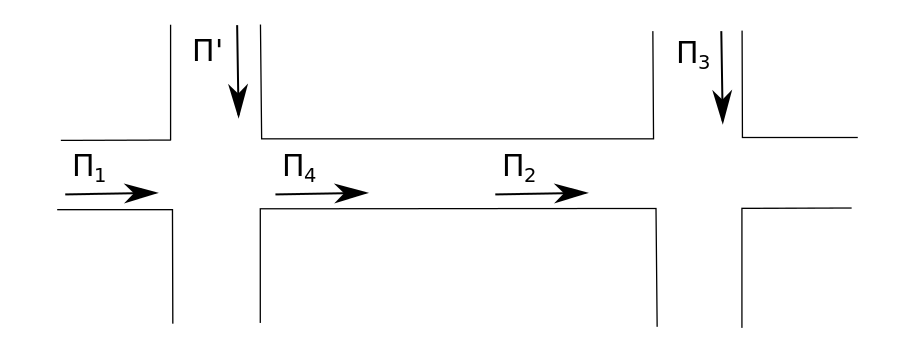
\includegraphics[scale=0.5]{Crossroads.png} 
\end{figure}

\begin{figure}[h]
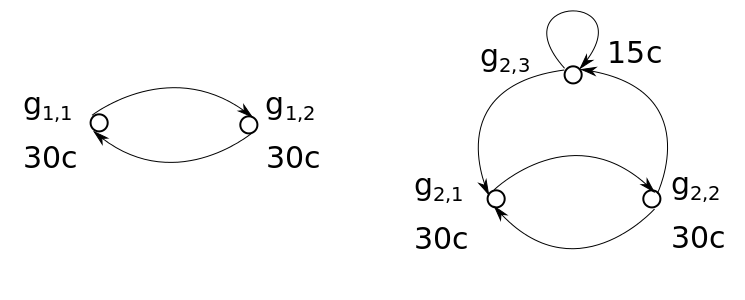
\includegraphics[scale=0.5]{SystemStates.png} 
\end{figure}



Требования по потокам $\Pi_j$, $j=1,2,4$, поступают пачками, причем пачки поступают в соответствии с Пуассоновским процессом с параметром $\la_j$. Требования из потока $\Pi_1$, будучи обслуженными, образуют поток $\Pi_3$.
Требования по потоку $\Pi_j$ поступают в соответствующую очередь $O_j$, $j=\overline{1,4}$.

Первый перекресток может находиться в одном из двух состояний:
\begin{itemize}
\item обслуживать поток $\Pi_1$ (состояние $\gam{1}{1}$ длительностью $\T{1}{1}$) и 
\item
обслуживать поток $\Pi_2$ (состояние $\gam{1}{2}$ длительностью $\T{1}{2}$).
\end{itemize}

Второй перекресток имеет три состояния:
\begin{itemize}
\item обслуживание потока $\Pi_3$ (состояние $\gam{2}{1}$ длительностью $\T{2}{1}$);
\item обслуживание потока $\Pi_4$ (состояние $\gam{2}{2}$ длительностью $\T{2}{2}$) и
\item продолжение обслуживания потока $\Pi_4$ в случае 
превышения объема оставшейся очереди $O_4$ некого порога (состояние $\gam{2}{3}$ длительностью $\T{2}{3}$);
\end{itemize}

Объединим рассматриваемые обслуживающие устройства в одно, состояние которого опишем с помощью вектора из множества $S_{general}\left(\Gamma^{(1,i_1)}; \Gamma^{(2,i_2)}; T\right)$, где $i_1\in \left\{1,2\right\}$, $i_2 \in \left\{1,2,3\right\}$, $T\in \left\{1, 2, \ldots, \max_{i_1,i_2}{\left(T^{(1,i_1)}, T^{(2,i2)}\right)}\right\}$. Свое состояние новое устройство меняет в моменты смены состояний одного из составляющих его устройств.

\begin{theorem}
Количество состояний полученного обслуживающего устройства конечно
\end{theorem}
\begin{proof}
Поскольку множество различных состояний $\Gamma$, в которые обслуживающее устройство может совершить переход, является подмножеством $S_{general}$ ($S \subset S_{general}$), то
\begin{equation*}
\left|S\right| \leqslant \left|S_{general}\right| = 2\times 3 \times \max_{i_1,i_2}{\left(T^{(1,i_1)}, T^{(2,i2)}\right)}
\end{equation*}
\end{proof}

В следствие этого результата мы можем перенумеровать состояния $\G = \brrr{\G^{(1)},\G^{(2)}, \ldots, \G^{(n)}}$, а также соответствующие им длительности $T=\brrr{T^{(1)},T^{(2)}, \ldots, T^{(n)}}$.
Каждое состояние $\G^{(r)}$ принадлежит одному из следующих четырех классов $\G^{\mathrm{\Rmnum{1}}}$, $\G^{\mathrm{\Rmnum{2}}}$, $\G^{\mathrm{\Rmnum{3}}}$ и $\G^{\mathrm{\Rmnum{4}}}$.
\begin{itemize}
\item в состоянии $\G^{(r)} \in \G^{\Rmnum{1}}$ обслуживаются только требования из очередей $O_1$ и $O_3$;
\item в состоянии $\G^{(r)} \in \G^{\Rmnum{2}}$ обслуживаются только требования из очередей $O_1$ и $O_4$;
\item в состоянии $\G^{(r)} \in \G^{\Rmnum{3}}$ обслуживаются только требования из очередей $O_2$ и $O_3$;
\item в состоянии $\G^{(r)} \in \G^{\Rmnum{4}}$ обслуживаются только требования из очередей $O_2$ и $O_4$.
\end{itemize}

Для описания процесса обслуживания будут также использоваться потоки насыщения $\Pi^{\mathrm{sat}}_j$, $j=\overline{1,4}$, определяемые как выходные потоки при максимальной загруженности обслуживающего устройства. Пусть
\begin{itemize}
\item для $j=1$ $^j\G=\G^{\Rmnum{1}} \cup \G^{\Rmnum{2}}$;
\item для $j=2$ $^j\G=\G^{\Rmnum{3}} \cup \G^{\Rmnum{4}}$;
\item для $j=3$ $^j\G=\G^{\Rmnum{1}} \cup \G^{\Rmnum{3}}$;
\item для $j=4$ $^j\G=\G^{\Rmnum{2}} \cup \G^{\Rmnum{4}}$;
\end{itemize}
Тогда поток насыщения $\Pi^{\mathrm{sat}}_j$ будет содержать неслучайное число $l_{r,j}$ требований, обслуженных в течение времени $\Tt{k,r}$, если $\ga{k,r} \in ^j\G$, и не будет содержать требований в противном случае, $\ga{k,r} \notin ^j\G$. 

Моменты $\tau_0 = 0, \tau_1, \ldots$ наблюдения за системой положим совпадающими с моментами переключения состояния обслуживающего устройства. Определим следующие случайные величины и элементы:
\begin{itemize}
\item количество $\vk_{j,i} \in Z_+ $ требований в очереди $O_j$ в момент времени $\tau_i$;
\item состояние обслуживающего устройства $\G_i\in \G = \brrr{\G^{(1)},\G^{(2)}, \ldots, \G^{(n)}}$ в течение $\left(\tau_{i-1};\tau_i\right]$;
\item количество $\eta_{j,i}$ требований, поступивших в очередь $O_j$ по потоку $\Pi_j$ в течение $\left(\tau_{i};\tau_{i+1}\right]$;
\item количество $\xi_{j,i}$ требований по потоку насыщения $\Pi^{\mathrm{sat}}_j$ в течение $\left(\tau_{i};\tau_{i+1}\right]$;
\item количество $\overline{\xi_{j,i}}$ реально обслуженных требований по потоку $\Pi_j$,
\end{itemize}
для $j=\overline{1,4}$.






В данной работе будет применен так называемый кибернетический подход, который предполагает, что наблюдение за системой осуществляется в дискретные моменты времени $\tau_0 = 0,~ \tau_1,~ \ldots$,~  совпадающие с моментами переключения состояния обслуживающего устройства. 
Будем считать, что функция перехода из состояния $\G_i$ в момент $\tau_i$ в состояние $\G_{i+1}$ в момент $\tau_{i+1}$ известна и задается функцией $h(\G_i,x_i)$ от предыдущего состояния $\G_i$ и величины $x_i$ очереди $O_3$ в момент $\tau_i$. Таким образом, обслуживающее устройство, в зависимости от объема очереди $O_3$, может переходить в разные состояния, что влечет за собой особый класс рассматриваемых графов переходов. Опишем сейчас общую структуру класса ${\cal K}$ рассматриваемых графов переходов между состояниями обслуживающего устройства (ОУ).

Первое и самое очевидное требование, которое мы наложим на рассматриваемый класс графов, --- это ориентированность и связность. Порядок прохождения состояний ОУ имеет значение и рассматривать недостижимые состояния (которые делают граф несвязным) не имеет смысла.

Далее, будем предполагать, что каждый граф $G$ из класса ${\cal K}$ может быть построен по следующему алгоритму.
\begin{enumerate}
\item Выделить из множества всех вершин графа $d$ непересекающихся кластеров вершин $C_1$, $C_2$, $\ldots$, $C_d$ таким образом, чтобы вершины внутри кластеров были соединены в цикл. Каждый кластер $C_j$ в свою очередь разделить на три непересекающихся множества вершин $C_j=C_j^{\mathrm{I}} + C_j^{\mathrm{O}} + C_j^{\mathrm{N}}$. Множество $C_j^{\mathrm{I}}$ будем называть множеством входных вершин, $C_j^{\mathrm{O}}$~--- множеством выходных вершин и $C_j^{\mathrm{N}}$~--- множеством нейтральных вершин. (Рис.~\ref{GraphSchemeOne}).

\begin{figure}[h]
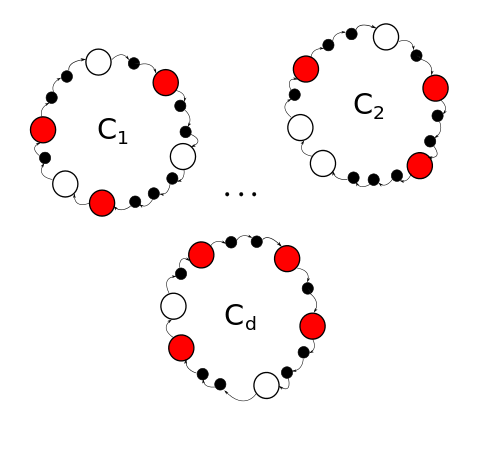
\includegraphics[scale=0.4]{GraphScheme1.png} 
\caption{Класс графов переходов (Шаг 1). Незакрашенные вершины --- выходные вершины, красным отмечены входные вершины, черным --- нейтральные}
\label{GraphSchemeOne}
\end{figure}
\item Каждое выходное состояние $c_1$ некоего кластера $C_j$ может быть соединено с входным состоянием того же или другого кластера $C_k$ постредством сторонней вершины $c$, не принадлежащей никакому из кластеров $C_1$, $C_2$, $\ldots$, $C_d$, и двух соединящих ребер (Рис.~\ref{GraphSchemeTwo}).
\begin{figure}[h]
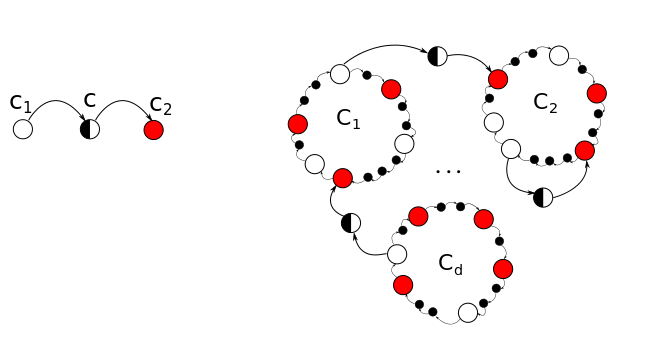
\includegraphics[scale=0.4]{GraphScheme2.png} 
\caption{Класс графов переходов (Шаг 2). Слева~--- шаблон соединения выходной и входной вершин. Справа~--- пример получаемого графа после шага 2. Полузакрашенные вершины~--- сторонние вершины, не принадлежащие ни одному кластеру $C_1$, $C_2$, $\ldots$ $C_d$}
\label{GraphSchemeTwo}
\end{figure}

\item Каждая сторонняя вершина, получаемая на шаге $2$, может быть соединена похожим образом с входной вершиной некоего кластера $C_j$: то есть посредством новой (еще не учавствовавшей в построении графа) сторонней вершины и двух новых ребер, или же посредством уже существующей сторонней (не входящей ни в один из кластеров) вершины и всего одного нового ребра (Рис.~\ref{GraphSchemeTree}).

\begin{figure}[h]
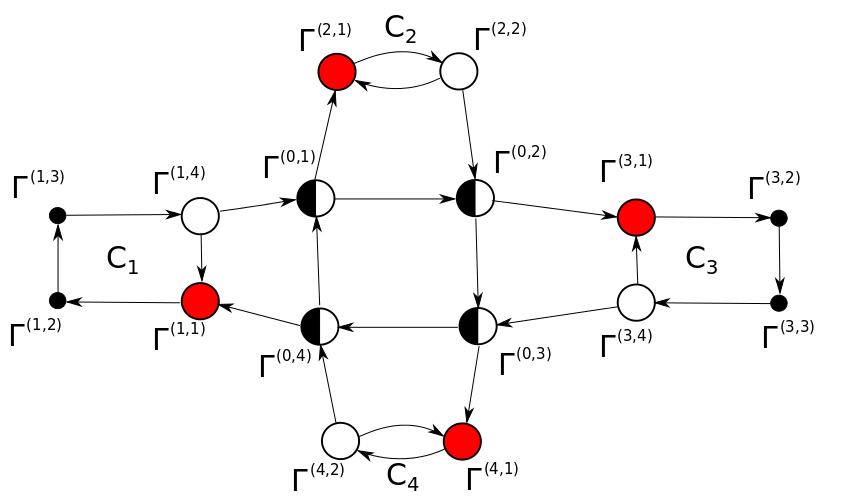
\includegraphics[scale=0.5]{GraphScheme3.png} 
\caption{Класс графов переходов (Шаг 3)}
\label{GraphSchemeTree}
\end{figure}
\end{enumerate}

Стоит отметить, что шаг $3$ может повторяться неоднократно, но конечное число раз.
 
Последнее требование, которое будет наложено заключается в следующем. Изо всех выходных вершин кластеров должны выходить ровно два ребра, ровно как во входные вершины кластеров должно входить также ровно два ребра; что касается сторонних вершин, то и из любой сторонней вершины должны выходить также по два ребра.
















\subsection{Кибернетический подход к изучению систем массового обслуживания с управлением}
Теперь перейдем к описанию основного метода, используемого в данной работе для исследования построенной модели. Не вдаваясь в данном разделе в математические детали, сформулируем основную задачу теории массового обслуживания и некоторые наиболее известные подходы к ее решению. 

Математической моделью системы обслуживания, как правило, является случайный процесс $\brrr{\xi(t) \colon t \in T}$ такой, что случайная величина $\xi(t)$ задает состояние системы в момент $t \in T$. Задача исследовтеля заключается в том, чтобы восстановить по физическому описанию системы вероятностное распределение этого процесса и изучить свойства распределения. Обозримость решения этой задачи во многом зависит от выбора описания состояния системы. В классических работах по данной тематике, например, изучались длина очереди, время ожидания начала обслуживания произвольного требования, число занятых линий. В связи с созданием и развитием А.А.~Боровковым асимптотических методов анализа в теории массового обслуживания в его работах система описывается трехмерным случайным процессом $\brrr{\eta(t), \nu(t), \zeta(t)\colon t \geqslant 0}$, в котором компоненты $\eta(t)$, $\nu(t)$ и $\zeta(t)$ соответственно определяют число поступивших, число получивших отказ и число обслуженных требований за промежуток $[0;t)$. 

Далее, кроме процесса $\brrr{\xi(t) \colon t \in T}$ рассматривают также процесс $\brrr{u(t) \colon t \in T}$, интерпретируемый как управление системой обслуживания. Управление может быть и случайным элементом, и детерменированной величиной. Ограничения на множество всех допустимых управлений имеют различную природу: математическую (например, измеримость), физическую (например, непрерывность), специфика задачи (например, в задачах о назначении приоритетов при обслуживании разнотипных требований).

Таким образом, математик -- исследователь управляемой системы массового обслуживания должен решать непростую задачу по описанию управляемого случайного процесса $\brrr{(\xi(t), u(t)) \colon t \in T}$. Упомянутые подходы обладают тем недостатком, существенно затрудняющими их применение для реальных систем, что достигаемая ими математическая общность не дает возможности принять в расчет многие физические особенности конкретных систем и построить конечномерные распределения рассматриваемого случайного процесса $\brrr{(\xi(t), u(t)) \colon t \in T}$.

В связи с вышесказанным, в данной работе будет применен другой подход, который с единых позиций рассматривает любую управляемую систему. Этот подход называется кибернетическим. Он базируется на трех постулатах. Во--первых, система массового обслуживания, как и многие другие кибернетические системы, функционирует в дискретном времени. Действительно, моменты поступления требований, моменты окончания обслуживания и другие события образуют дискретную совокупность точек на временной оси. Поэтому следует в первую очередь выбрать дискретную временную шкалу $T=\brrr{\tau_0, \tau_1, \ldots}$ и привязывать к ней все другие рассматриваемые величины и объекты. 

Во--вторых, описание состояния элементов системы в любой момент времени $t \geqslant 0$ даже для простых законов распределения входных потоков и длительностей обслуживания приводит к сложным математическим проблемам. Локальный принцип не учитывает в полной мере физическую природу процесса обслуживания и такие важные возможности и особенности действующих систем, как функции ориентации и переналадок, неоднородность требований, изменчивость с течением времени вероятностной структуры входных потоков и длительностей обслуживания, адаптивность логической структуры обслуживающего устройства, наконец, конфликтность ситуаций в управлении и обслуживании. Итак, описание поэлементного строения системы должно быть нелокальным.

В--третьих, следует выбрать уровень детализации, на котором рассматривается система. Исторически первым был метод анализа и синтеза. Сложная система мысленно расчленялась на свои составляющие и каждая часть изучалась отдельно во всей своей полноте. Затем знание обо всех частях соединялось, синтезировалось в знание обо всей совокупности, объединенной в систему. Проблемы, возникающие при таком подходе, уже обсуждались выше. Это и огромное число составляющих, и невозможность полного описания одной части без учета ее взаимодействия с другими частями. Другой подход, появившийся лишь в $\mathrm{\Rmnum{20}}$ веке, носит название <<черный ящик>>. Исследователь вовсе не интересуется устройством системы, а пытается лишь подобрать зависимость <<выхода>> системы от ее <<входа>>. Напротив, кибернетический подход отдает дань умеренности. Считается, что каждая управляемая система обладает схемой, на которой присутствуют элементы небольшого числа типов: 1) внешняя среда, 2) полюса --- точки взаимодействия системы со средой, 3) внешняя и внутренняя память, 4) устройства по переработке информации во внешней и внутренней памяти. Память состоит из ячеек с дискретным множеством состояний. Информацией является совокупность состояний всех ячеек памяти в данный момент времени. Расположение элементов на схеме описывают координаты. Благодаря им система может воздействовать на саму себя в соответствии со своими функциональными свойствами. Функция системы определяет поведение системы массового обслуживания. Она указывает то действие, которое система может совершать, переходя к следующему моменту времени. Таким образом, под состоянием $\xi(\tau)$ системы можно понимать состояния указанных элементов в момент времени $\tau \in T$, и требуется формализовать функцию системы путем совместного рассмотрения поэлементного строения системы и ее функционирования во времени. 

Более подробно и применительно к рассматриваемой задаче кибернетический подход будет описан в следующих разделах. Будет построена математическая модель управляемой системы массового обслуживания в виде счетных управляемых марковских цепей.

















Все рассматриваемые в этой работе случайные элементы определяются на общем вероятностном пространстве $\br{\Omega, {\cal F}, P}$ элементарных исходов $\omega \in \Omega$ с вероятностной мерой $P(A)$, $A \in {\cal F}$, на $\sigma$-алгебре ${\cal F}$. 

Введем следующие случайные величины и элементы, $j \in \brrr{1,2,3,4}$:
\begin{itemize}
\item количество $\vk_{j,i} \in Z_+ $ требований в очереди $O_j$ в момент времени $\tau_i$;
\item состояние обслуживающего устройства $\G_i\in \G = \brrr{\G^{(1)},\G^{(2)}, \ldots, \G^{(n)}}$ в течение времени $\left(\tau_{i-1};\tau_i\right]$;
\item количество $\eta_{j,i}$ требований, поступивших в очередь $O_j$ по потоку $\Pi_j$ в течение времени $\left(\tau_{i};\tau_{i+1}\right]$;
\item количество $\xi_{j,i}$ требований по потоку насыщения $\Pi^{\mathrm{sat}}_j$ в течение времени $\left(\tau_{i};\tau_{i+1}\right]$;
\item количество $\overline{\xi}_{j,i}$ реально обслуженных требований по потоку $\Pi_j$ в течение времени $\left(\tau_{i};\tau_{i+1}\right]$.
\end{itemize}

Тогда для $j \in \brrr{1,2,3}$ имеем
\begin{equation}
\G_{i+1}=h(\G_i,\vk_{3,i}),\quad \vk_{j,i+1}=\max{\brrr{0,\vk_{j,i}+\eta_{j,i}-\xi_{j,i}}}, \quad \overline{\xi}_{j,i} = \min{\brrr{\xi_{j,i},\vk_{j,i}+\eta_{j,i}}}
\label{deterministicLawOne}
\end{equation}
и 
\begin{equation}
\eta_{2,i} = \overline{\xi}_{4,i}, \quad \eta_{4,i}=\overline{\xi}_{1,i}, \quad \vk_{4,i+1}=\vk_{4,i} + \overline{\xi}_{1,i} - \overline{\xi}_{4,i}
 \label{deterministicLawTwo}
\end{equation}
Также для определения длительности $T_{i}$ состояния обслуживающего устройства в течение $\left(\tau_{i-1};\tau_i\right]$, удобно ввести функцию $h_T(\cdot,\cdot)$:
\begin{equation}
T_{i+1}=h_T(\G_i,\vk_{3,i})= \Tt{r'},\quad  \text{ где } \ga{r'}=h(\G_i,\vk_{3,i}).
\label{timeLaw}
\end{equation}

Обозначим через $\vp_j(x,t)$, $j\in \brrr{1,3}$, условную вероятность того, что за время $t>0$ по потоку $\Pi_j$ поступит ровно $b\in Z_+$ требований:
\begin{equation}
\P{ \eta_{j,i} = b}{\G_i=\ga{k,r}, \vk_{3,i}=x}=\vp_j(b,h_T (\ga{k,r}, x)).
\end{equation}
Учитывая закон распределения процесса Пуассона и количества требований в пачках, величины $\vp_j(x,t)$ могут быть найдены из соотношений
\begin{equation}
\sum_{x=0}^{\infty} z^x\vp_j(x,t) = \exp\brrr{\la_j t \br{\sum_{b=1}^{\infty} z^b \pi(b,j) -1}}.
\end{equation}

Для потоков насыщения имеем следующие соотношения:
\begin{align}
\P{\xi_{j,i} = 0}{\G_i=\ga{k,r}, \vk_{3,i} = x} = 1, &\quad \G_{i+1} \notin~^j\G,\\
\P{\xi_{j,i} = \ell_{r',j}}{\G_i=\ga{k,r}, \vk_{3,i} = x} = 1, &\quad \G_{i+1}=\ga{r'}\in~^j\G,
\end{align}
где $j\in \{1, 2, 3\}$, $x \in Z_+$.


Введем для $0 < u \leqslant 1$ и $0 \leqslant k \leqslant x$ величину
\begin{equation}
\psi\br{k,x,u} = C_x^k u^k (1-u)^{x-k}.
\end{equation}
Поскольку требования из очереди $O_4$ независимо друг от друга с вероятностью $p_{k,r}$ на выходе системы поступают в очередь $O_2$, то количество требований в выходном потоке $\Pi_4^{\mathrm{\text{вых}}}$ определяется по биномиальному закону распределения:
\begin{equation}
\P{\overline{\xi}_{4,i} = b}{ \G_i = \ga{k,r}, \vk_{4,i}=x, \vk_{3,i}=\tilde{x}}=\psi\br{b,x,p_{r'}}, \quad \G_{i+1}=\ga{r'}, \quad 0 \leqslant b \leqslant x.
\end{equation}












































Изучим теперь свойства распределения $P(\cdot)$ построенного вероятностного пространства $(\Omega,{\cal F},P(\cdot))$ и, в частности, убедимся в том, что оно отражает основные характеристики рассматриваемой системы массового обслуживания.

Начнем со связи последовательности $X(\omega)=(X_0(\omega), X_1(\omega),\ldots)$ со случайными величинами из \eqref{functionsOne}, \eqref{functionsTwo}, \eqref{functionsThree}. Поскольку (см. \eqref{ProbabilitiesGeneralOne} и \eqref{ProbabilitiesGeneralTwo}) 
\begin{equation*}
P(X_0(\omega)=a_0) = P_0(\eta_0(\omega_0)=a_0) 
\end{equation*}
и
\mll
{\P{X_n(\omega)=a_n}{X_0(\omega) = a_0, X_1(\omega)=a_1,\ldots, X_{n-1}(\omega)=a_{n-1}} = \\
= P_n(a_0,a_1,\ldots, \{\eta_n(\omega_n)=a_n\}),
}
то условные распределения случайных величин $X_n(\omega)$ и распределения случайных величин $\eta_n(\omega_n)=(\eta_{1,n}(\omega_n),\eta_{2,n}(\omega_n),\eta_{3,n}(\omega_n))$ совпадают, $n\geqslant 0$. Таким, образом, $X_n(\omega)$ можно рассматривать как <<продолжение>> величин $\eta_n(\omega_n)$ на общее вероятностное пространство $(\Omega,{\cal F},P(\cdot))$ с исходных пространств $(\Omega_n,{\cal F}_n,P_n(\omega_0,\omega_1,\ldots,\omega_{n-1},\cdot))$. Тогда определенные в прошлом разделе на качественном уровне величины теперь можно определить формально:
	
\begin{equation}
\begin{aligned}
\eta_{j,n}(\omega) &= X_{j,n}(\omega),\quad \overline{\xi}_{4,0}(\omega)=\eta_{2,0}(\omega), & \quad \G_{i+1}(\omega)&=h(\G_{i}(\omega),\vk_{3,i}(\omega)),\\
\vk_{j,i+1}(\omega)&=\max{\left\{ 0,\vk_{j,i}(\omega)+\eta_{j,i}(\omega) - \xi_{j,i}(\omega)\right\}},& \quad
\xi_{j,i}(\omega)&=f_{\xi_j | \G,\vk_3} (\G_i(\omega),x_{3,i}(\omega)),
\end{aligned}
\label{RandomVariablesOne}
\end{equation}
и
\begin{equation}
\vk_{4,i+1}(\omega)=\vk_{4,i}(\omega)+\eta_{4,i}(\omega -\overline{\xi}_{4,i}(\omega)),\quad
\eta_{4,i}(\omega)=f_{\eta_4| \xi_1, \eta_1, \vk_1} (\xi_{1,i}(\omega),\eta_{1,i}(\omega),\vk_{1,i}(\omega)),
\label{RandomVariablesTwo}
\end{equation}
Где $\G_0=\gamma_0=\mathrm{const}$ и $\vk_0=(\vk_{1,0},\vk_{2,0},\vk_{3,0},\vk_{4,0})=(x_{1,0},x_{2,0},x_{3,0},x_{4,0})=\mathrm{const}$.
Величины, определенные в \eqref{RandomVariablesOne} и \eqref{RandomVariablesTwo}, являются случайными величинами, поскольку выражаются через конечное число случайных величин $X_{j,n}(\omega)$, $j\in\{1,2,3\}$, $n\geqslant 0$. Причем 
\mll
{
\P{\eta_{j,n}(\omega)=a_{j,n}}{\eta_{0}(\omega)=a_0,\eta_{1}(\omega)=a_1,\ldots, \eta_{n-1}(\omega)=a_{n-1}} =\\ = \P{X_{j,n}(\omega)=a_{j,n}}{X_0(\omega) = a_0, X_1(\omega)=a_1,\ldots, X_{n-1}(\omega)=a_{n-1}} =\\= \vp_j(a_{j,n},h_T(\G_n(\omega),\vk_{3,n}(\omega)))
}
для $j\in\{1,3\}$ и 
\mll
{
\P{\eta_{2,n}(\omega)=a_{2,n}}{\eta_{0}(\omega)=a_0,\eta_{1}(\omega)=a_1,\ldots, \eta_{n-1}(\omega)=a_{n-1}} =\\ = \P{X_{2,n}(\omega)=a_{2,n}}{X_0(\omega) = a_0, X_1(\omega)=a_1,\ldots, X_{n-1}(\omega)=a_{n-1}} =\\= \begin{cases} \binom{x}{a} p_{k,r}^a(1-p_{k,r})^{x-a}, \quad &\text{если } h(\G_n(\omega),\vk_{3,n}(\omega))=\ga{k,r}, \vk_{4,n}(\omega)=x \\ 0, \quad &\text{иначе}\end{cases}
}
что соответствует вероятностным предпосылкам, заложенным в описание рассматриваемой системы массового обслуживания.
%Учитывая \eqref{probabilitiesTwo}, распишем
%\ml
%{
%P_{n+1}(\omega_0,\omega_1,\ldots,\omega_n,\brrr{\eta_{1,n+1}(\omega_{n+1}) = a_1}) = P_{n+1}(\omega_0,\omega_1,\ldots,\omega_n,\brrr{\omega_{1,n+1} = a_1})=\\
%= \sum_{a_2,a_3 \in Z_+}P_{n+1}(\omega_0,\omega_1,\ldots,\omega_n,\brrr{(\omega_{1,n+1},\omega_{2,n+1},\omega_{3,n+1}) = (a_1,a_2,a_3)})
%}
%

%В первую очередь, определим, чему соответствует последовательность $X(\omega)=\br{X_1(\omega),X_2(\omega),\ldots}$. 


